\section{3-Schicht-System aus Cu und Fe}
\subsection{Probendesign}
In diesem Abschnitt wird die Möglichkeit erörtert in einem 3-Schicht-System die Cu-$L$-Kante zur Fluoreszenz anzuregen und den Kontrast in der Absorption durch eine darüber liegende Fe-Lackschicht bzw. eine Lackschicht ohne schwere Elemente zu detektieren.

Diese Möglichkeit kann in Betracht gezogen werden, falls an einer Beamline mit im Bereich von \SI{1.1}{\kilo\electronvolt} Photonenenergie gearbeitet wird und die Präparation von 2 Ebenen übereinander gelingt. \newline
Die chemischen Kompositionen des vorangegangenen Kapitels werden beibehalten. Auf dem $Si_3N_4$-Fenster befindet sich nun eine weitere, durchgehende Lackschicht, in welche Kupfer mit einem Massenanteil von knapp 6\% eingemischt ist. Diese bildet die mittlere Ebene des Probendesigns. Die Dichte der $C_{64}H_{56}O_{12}Cu$-Schicht wird durch Gewichtung der Massenanteile und Dichten von Lack und Kupfer zu \SI{1.35}{\gram\per\cubic\centi\meter} geschätzt. Damit ergibt sich, ausgehend von einer Transmission von unter 20\%, eine Schichtdicke von \SI{5}{\micro\meter}. Die Abschätzung der Absorption der prägnanten Cu-$L_{{\alpha}2}$ und $L_{{\beta}1}$ durch die Fe-Lackschicht mit Hilfe des CRXO-Tools liefert für die gewünschte Länge des längeren Absorptionspfad $c_a = \SI{4.5}{\micro\meter}$, respektive für den kürzeren Absorptionspfad $c_i = \SI{3.2}{\micro\meter}$, sodass im Mittel etwa 25\% der eintreffenden Fluoreszenzstrahlung transmittieren sollten. Daraus errechnet sich nach \cref{eq:h} die Schichthöhe zu abgerundet zu $h = \SI{2.5}{\micro\meter}$, nach \cref{eq:rp} folgt aufgerundet für die Schichtbreite $r_p = \SI{3.7}{\micro\meter}$. Dies ist in \cref{tab:cu_fe} zusammengefasst.

 \begin{table}[H]
 \centering
 \begin{tabular}{|c|c|c|c|c|} \hline
  Ebene & chem. Komposition & Dichte & Höhe & Breite	\\ \hline
  0 & $C_{16}H_{14}O_{3}$ 		& \SI{0.87}{\gram\per\cubic\centi\meter}	& \SI{2.5}{\micro\meter} & \SI{3.7}{\micro\meter} \\ \hline
  0 & $C_{64}H_{56}O_{12}Fe$	& \SI{1.22}{\gram\per\cubic\centi\meter}	& \SI{2.5}{\micro\meter} & \SI{3.7}{\micro\meter} \\ \hline
  1 & $C_{64}H_{56}O_{12}Cu$	& \SI{1.35}{\gram\per\cubic\centi\meter}	& \SI{5}{\micro\meter} & \SI{25.9}{\micro\meter} \\ \hline
  2 & $Si_{3}N_{4}$				& \SI{3.17}{\gram\per\cubic\centi\meter}	& \SI{200}{\nano\meter} & \SI{25.9}{\micro\meter} \\ \hline
 \end{tabular}
   \caption{Tabellarisch sind die Parameter der einzelnen Schichten für die Anregung der Cu-$L$-Kante bei \SI{1.1}{\kilo\electronvolt} und Absorption in einer höher liegenden Schicht an der Fe-$L$-Kante aufgelistet.}
 \label{tab:cu_fe}
 \end{table}
 
Abschließend soll die Möglichkeit betrachtet werden die Probe mittels Transmissions\-spektroskopie zu untersuchen. Dafür muss die Transmission der Synchrotronstrahlung durch die leichte Lackschicht und das Siliziumfenster berechnet werden. Es ergibt sich, dass die Synchrotronstrahlung zu knapp 65\% durch die leichte Lackschicht und zu etwa 90\% durch das Siliziumfenster transmittiert. Zusammen mit dem für die Kupferschicht bestimmten Wert von 20\% ergibt sich eine Restintensität von über 10\% welche zu vergleichenden Untersuchungen durch Transmissions"=spektroskopie genutzt werden können.

\subsection{Simulation}
\begin{figure}[H] 
  \centering
     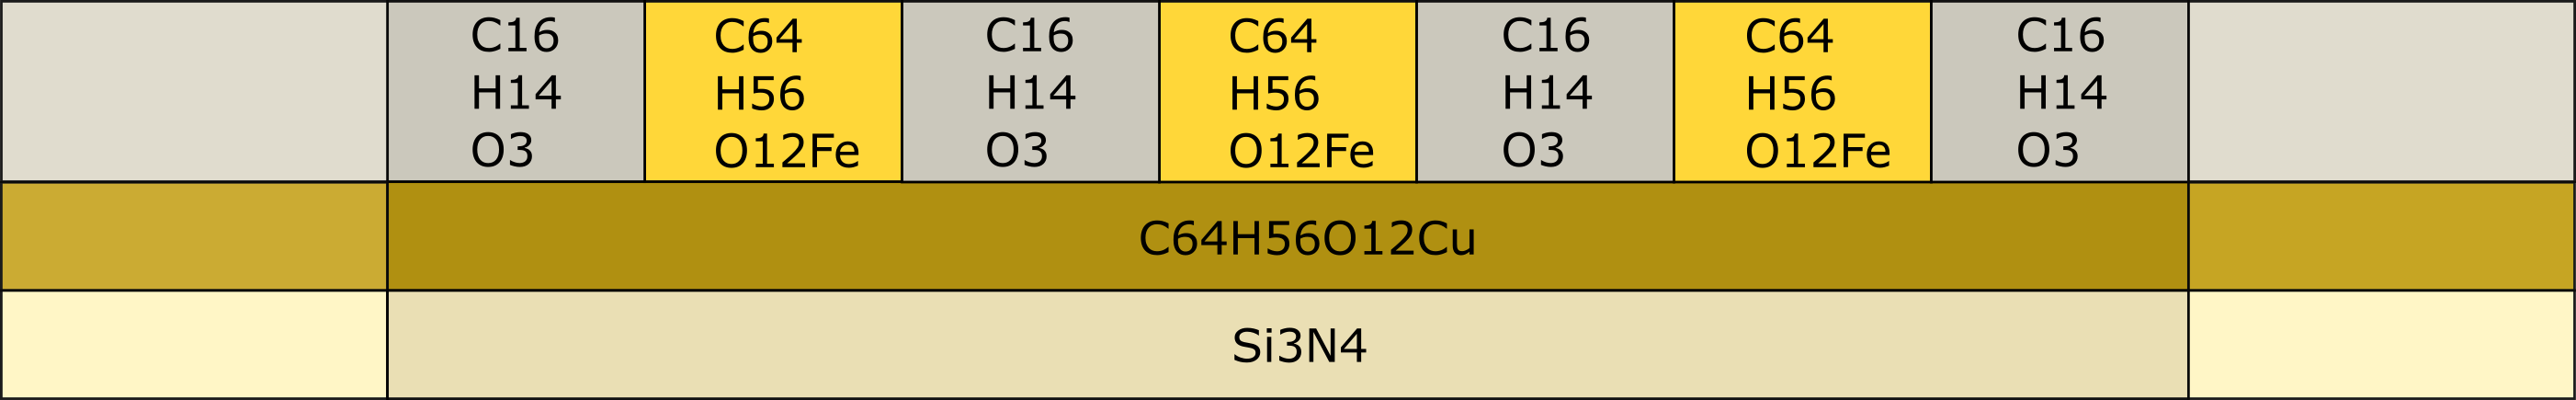
\includegraphics[width=1\textwidth]{illustrations/cu_unter_fe.png}
  \caption[Probendesign Kupferkante]{Querschnitt durch die Probe: Auf einem Siliziumnitridfenster befindet sich eine durchgehende Ebene mit beigemischten Cu-Partikeln. Darüber die bereits bekannte, sich abwechselnde Struktur, aus Lacken mit und ohne Fe-Partikeln. Der Bereich außerhalb des späteren Scanbereichs ist an den Rändern etwas aufgehellt und unbeschriftet dargestellt.}
  \label{fig:cu_unter_fe}
\end{figure}

Damit genug Messpunkte im interessanten Bereich an den Schichtgrenzen liegen ist die Schrittweite aufgrund der deutlich kürzeren Gesamtbreite der Probe in dieser Simulation auf \SI{100}{\nano\meter} nach unten korrigiert worden. Alle anderen in \cref{sec:vorwort} gelisteten Parameter wurden unverändert beibehalten. Die Anregungsenergie beträgt \SI{1.1}{\kilo\electronvolt}. Eine Illustration des detektierten Eisen- (\cref{fig:cu_fe_fe_signal}) und des Kupfersignals (\cref{fig:cu_fe_cu_signal}) ist im Folgenden dargestellt.

\begin{figure}[H] 
  \centering
     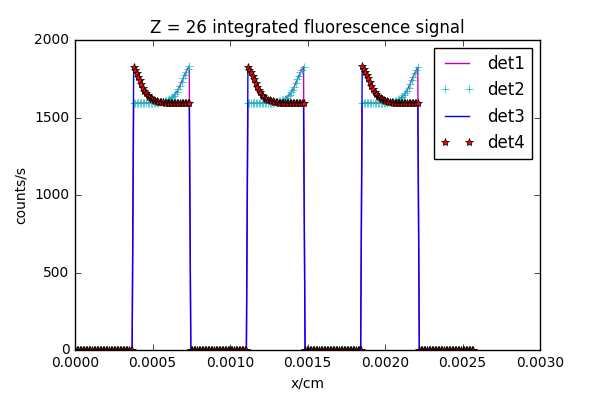
\includegraphics[width=0.85\textwidth]{illustrations/cu_fe_fe_signal.png}
  \caption[Simuliertes Eisensignal über Kupferkante]{Abgebildet ist das simulierte Fluoreszenzsignal von Eisen beim Abrastern von zwei alternierenden homogenen Schichten. Über die x-Achse ist der Verlauf der detektierten Fluoreszenzintensität aufgetragen, welche außerhalb der Fe-Schichten 0 beträgt. An den Schichtgrenzen entstehen, je nach Detektororientierung, Maxima, der dahinter liegende Abfall wird durch Selbstabsorption in der Eisenschicht bedingt. }
  \label{fig:cu_fe_fe_signal}
\end{figure}

In \cref{fig:cu_fe_fe_signal} ist das simulierte Fe-Fluoreszenzsignal einer alternierenden Schichtfolge aus leichtem Lack und Fe-Lack abgebildet. Da nur Primärfluoreszenz betrachtet wird, kann nur dort ein Fe-Fluoreszenzsignal simuliert werden, wo Eisen enthalten ist. Daher ist in der leichten Lackschicht keine Fe-Fluoreszenz berechnet und beim Wechsel von leichter Lackschicht in den Fe-Lack ein Sprung zur maximalen Intensität sichtbar. Daraufhin kommt es zu Selbstabsorptionseffekten in der Fe-Lackschicht. Das Signal ist an der Schichtgrenze maximal und nimmt in die Schicht hinein etwas ab. Dies liegt daran, da Fluoreszenz, welcher weiter (in x-Richtung) in der Schicht emittiert wird, durch die Eisenschicht transmittieren muss, welche stärker absorbiert als die leichte Lackschicht. Da dies an den Schichtgrenzen auch für die detektierte Fluoreszenzstrahlung der gegenüberliegenden Detektoren gilt, ist für diese das Signal dort minimal bezüglich der Intensitäten der Fe-Schicht. Aufgrund der räumlichen Positionierung der Detektoren sind die Signale für Detektor 1+2 und Detektor 3+4 symmetrisch. \newline

Ausgehend von $x=\SI{0}{\micro\meter}$ wird der Verlauf des Cu-Fluoreszenzsignals (\cref{fig:cu_fe_cu_signal}) für die Detektoren 3+4 beschrieben. Von einer Beschreibung der Signale für die Detektoren 1+2 wird abgesehen, da die Begründungen äquivalent sind und sich nur der Beobachtungspunkt ändert, siehe \cref{fig:si_fe_si_signal}.

\begin{figure}[H] 
  \centering
     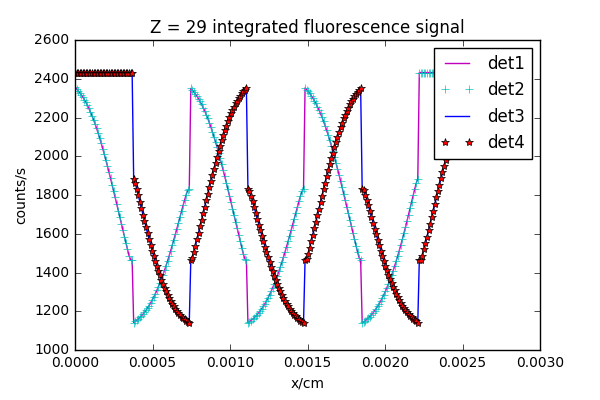
\includegraphics[width=0.85\textwidth]{illustrations/cu_fe_cu_signal.png}
  \caption[Simuliertes Kupfersignal über Kupferkante]{Detektiertes Cu-Fluoreszenzsignal der Detektoren 1-4. Das über die x-Achse aufgetragene Cu-Fluoreszenzsignal wird den einzelnen Detektoren zugeordnet. Die Kurvenverläufe sind durch die darüber liegenden, alternierende Schichten bedingt.}
  \label{fig:cu_fe_cu_signal}
\end{figure}

Beim Abrastern der ersten Schicht bis $x=\SI{3.7}{\micro\meter}$ wird ein konstantes Signal von etwa \SI{2400}{Counts \per\second} detektiert, da das Fluoreszenzsignal, welches in der darunter liegenden Kupferschicht angeregt wird keiner Absorption durch die Fe-Lackschicht ausgesetzt ist. Bei $x=\SI{0}{\micro\meter}$ transmittiert die Cu-Fluoreszenz vollständig durch die leichte Lackschicht, welche außerhalb des Scanbereichs liegt (siehe \cref{fig:cu_unter_fe}). Bei $x=\SI{3.7}{\micro\meter}$ fällt die detektierte Intensität abrupt auf etwa \SI{1900}{Counts \per\second} ab. Hauptsächlich liegt dies vermutlich an der erhöhten Abschwächung der Anregungsstrahlung in der Fe-Lackschicht im Gegensatz zur Lackschicht ohne Fe-Partikel. Die transmittierte Anzahl der Photonen mit \SI{1.1}{\kilo\electronvolt} bei einer Fe-Schichtdicke von \SI{2.5}{\micro\meter} beträgt etwa 50\%. Verglichen mit den 65\%, die durch die leichte Lackschicht gleicher Höhe transmittieren, entspricht dies einer Differenz von 15\% und somit einem relativen Abfall von etwa $\frac{15}{65} \approx \frac{1}{4}$ der gemessenen Intensität. Dies entspricht in etwa der Größenordnung der Intensitäten ($\frac{2400}{1900} \approx \frac{1}{4}$), welche in \cref{fig:cu_fe_cu_signal} dargestellt sind. Im weiteren Verlauf durch die nachfolgende Fe-Lackschicht ($x=3.7-\SI{7.4}{\micro\meter}$) fällt das detektierte Fluoreszenzsignal bedingt durch die Absorption in der Fe-Lackschicht weiter ab. An ihrem Minimum bei $x=\SI{7.4}{\micro\meter}$ ist die Absorption der Fluoreszenz maximal und es werden etwa \SI{1100}{Counts \per\second} gemessen. Direkt dahinter ist erneut ein Intensitätsprung beobachtbar. Die Begründung verläuft analog zum Sprung bei $x=\SI{3.7}{\micro\meter}$, jedoch steigt hier die Intensität. Nachfolgend steigt das detektierte Fluoreszenzsignal erneut an, da sich der Absorptionsweg durch Fe-Lackschicht immer weiter verkürzt und die Strahlung stattdessen durch die leichte Lackschicht transmittiert. Das Ansteigen des Fluoreszenzsignals endet in einem Maximum bei $x=\SI{11.1}{\micro\meter}$. Hier ist zu erkennen, dass das Fluoreszenzsignal noch nicht in der Sättigung angekommen ist. Vermutlich liegt dies daran, dass die z-Schrittweite $\Delta z$ für die Probe zu groß gewählt wurde. Der weitere Verlauf ist analog zu dem gerade Erläuterten beschreibbar. \newlines
Zusammenfassend ist zu sagen, dass auch hier die gewünschten Absorptionseffekte unter diesen Simulationsbedingungen stark ausgeprägt sind. Außerdem kann die Auswertung des Fe-Fluoreszenzsignals einen weiteren Hinweis darauf liefern, ob die zu erwartenden Selbstabsorptionseffekte auch in der Realität nachweisbar sind. Steht eine Beamline im Bereich von \SI{1.1}{\kilo\electronvolt} zur Verfügung ist diese Probe für eine experimentelle Untersuchung am Synchrotron zu empfehlen.